\begin{frame}
	\frametitle{\secname}

	\begin{theorem}
		If $\theta\in\mathds{R}$, then
		\begin{equation*}
			\operatorname{Im}
			\left(
			\sum\limits_{k=1}^{n}
			e^{i\left(2k-1\right)\theta}
			\right)=
			\sum\limits_{k=1}^{n}
			\operatorname{Im}
			\left(
			e^{i\left(2k-1\right)\theta}
			\right)=
			\sum\limits_{k=1}^{n}
			\sin\left(\left(2k-1\right)\theta\right)=
			\begin{cases}
				\dfrac{\sin^{2}\left(n\theta\right)}{\sin\left(\theta\right)},
				 & \exists m\in\mathds{Z}
				\text{ such that }\theta\neq 2m\pi. \\
				0,
				 & \text{otherwise}.
			\end{cases}
		\end{equation*}
	\end{theorem}

	\begin{proof}
		Since
		\begin{math}
			\sum\limits_{k=1}^{n}
			{\left(e^{i\theta}\right)}^{k}=
			e^{i\left(n+1\right)\frac{\theta}{2}}
			\frac{
				\sin\left(n\frac{\theta}{2}\right)
			}{
				\sin\left(\frac{\theta}{2}\right)
			}
		\end{math}:

		\begin{align*}
			\sum\limits_{k=1}^{n}
			{
			\left(
			e^{i\theta}
			\right)
			}^{2k-1}
			        & =
			e^{-i\theta}
			\alert{
			\sum\limits_{k=1}^{n}
			{
			\left(
			e^{i2\theta}
			\right)
			}^{k}
			}=
			e^{-i\theta}
			\alert{e^{i\left(n+1\right)\theta}}
			\frac{
				\alert{\sin\left(n\theta\right)}
			}{
				\alert{\sin\left(\theta\right)}
			}=
			e^{in\theta}
			\frac{\sin\left(n\theta\right)}{\sin\left(\theta\right)}.
			\shortintertext{
				Taking the \alert{imaginary part} on the opposite sides of
				the equality:
			}
			\operatorname{Im}
			\left(
			\sum\limits_{k=1}^{n}
			e^{i\left(2k-1\right)\theta}
			\right) & =
			\sin\left(n\theta\right)
			\frac{\sin\left(n\theta\right)}{\sin\left(\theta\right)}=
			\frac{\sin^{2}\left(n\theta\right)}{\sin\left(\theta\right)}.
		\end{align*}
	\end{proof}
\end{frame}

\begin{frame}
	\frametitle{\secname}

	\begin{columns}
		\begin{column}{0.42\textwidth}
			\begin{figure}
				\centering
				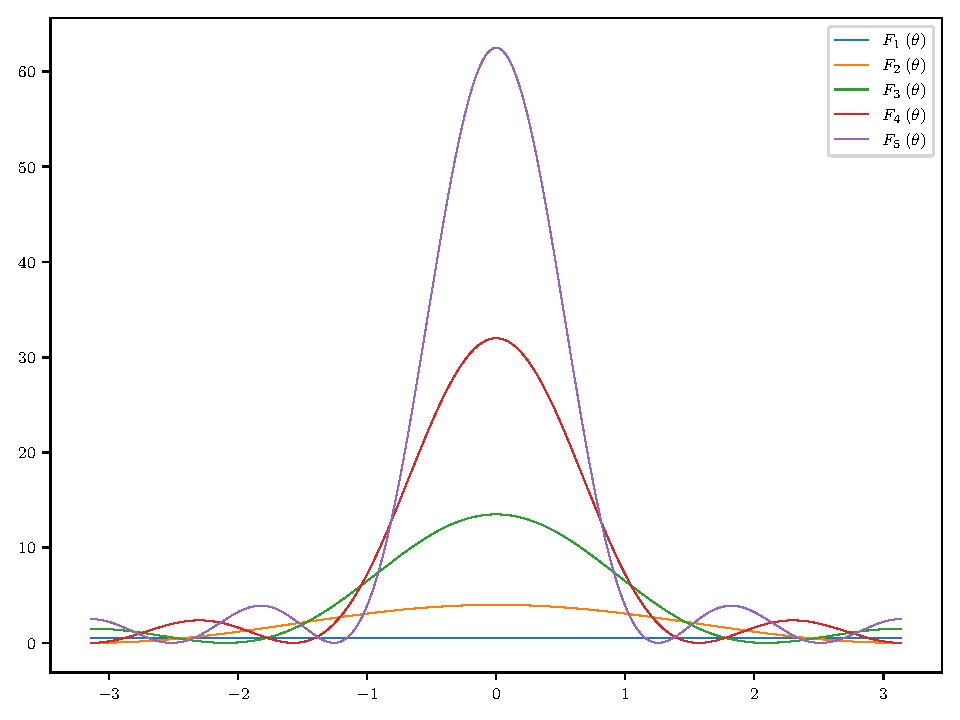
\includegraphics[width=0.35\paperwidth]{plot_fejer}
			\end{figure}
		\end{column}
		\begin{column}{0.54\textwidth}
			\begin{definition}[Fejér kernel]
				The \alert{Fejér kernel} $K_{n}$ of $n$-order is
				\begin{equation*}
					\fcolorbox{DarkBlue}{yellow}{
						\begin{math}
							\displaystyle
							K_{n}\left(\theta\right)\coloneqq
							\frac{1}{n}
							\sum_{k=1}^{n}D_{k-1}\left(\theta\right)
						\end{math}
					}
				\end{equation*}
				i.e. is the $n$-th Cesàro-Fourier means of the Dirichlet
				kernel.
			\end{definition}
		\end{column}
	\end{columns}

	\begin{definition}[$n$-th Cesàro-Fourier means]
		Let
		\begin{math}
			f\in L^{2}\left(\left[0,2\pi\right]\right)
		\end{math}.
		The \alert{$n$-th Cesàro-Fourier means} of $f$ is
		\begin{equation*}
			\fcolorbox{DarkBlue}{yellow}{
				\begin{math}
					\displaystyle
					\sigma_{n}f\left(\theta\right)=
					\frac{1}{n}\sum_{k=1}^{n}
					s_{k-1}f\left(\theta\right).
				\end{math}
			}
		\end{equation*}
	\end{definition}
\end{frame}

\begin{frame}
	\frametitle{\secname}

	\begin{lemma}
		If $f\in L\left(\left[0,2\pi\right]\right)$ is $2\pi$-periodic
		and $\left\{s_{n}f\left(\theta\right)\right\}_{n\in\mathds{N}}$
		is the sequence of partial sum of the trigonometric Fourier
		series generated by $f$.
		Then, the sequence
		\begin{math}
			\sigma_{n}
			f\left(\theta\right)
		\end{math}
		has the integral representation
		\begin{equation*}
			\fcolorbox{DarkBlue}{yellow}{
				\begin{math}
					\displaystyle
					\sigma_{n}f\left(\theta\right)=
					\frac{2}{\pi}
					\int\limits_{0}^{\pi}
					\frac{f\left(\theta+\xi\right)+f\left(\theta-\xi\right)}{2}
					K_{n}\left(\xi\right)\dl\xi.
				\end{math}
			}
		\end{equation*}
	\end{lemma}

	\begin{proof}
		If
		\begin{math}
			s_{n}f\left(\theta\right)=
			\displaystyle
			\frac{2}{\pi}
			\int\limits_{0}^{\pi}
			\frac{f\left(\theta+\xi\right)+f\left(\theta-\xi\right)}{2}
			D_{n}\left(\xi\right)\dl\xi
		\end{math},
		then
		\begin{align*}
			\sigma_{n}f\left(\theta\right)
			 & =
			\dfrac{1}{n}
			\sum\limits_{k=1}^{n}
			\alert{s_{k-1}f\left(\theta\right)}
			= \frac{1}{n}
			\sum\limits_{k=1}^{n}
			\alert{
				\frac{2}{\pi}
				\int\limits_{0}^{\pi}
				\frac{f\left(\theta+\xi\right)+f\left(\theta-\xi\right)}{2}
				D_{k-1}\left(\xi\right)\dl\xi
			}.   \\
			\sigma_{n}f\left(\theta\right)
			 & =
			\frac{2}{\pi}
			\int\limits_{0}^{\pi}
			\frac{f\left(\theta+\xi\right)+f\left(\theta-\xi\right)}{2}
			\alert{
				\frac{1}{n}\sum\limits_{k=1}^{n}
				D_{k-1}\left(\xi\right)
			}
			\dl\xi
			=
			\frac{2}{\pi}
			\int\limits_{0}^{\pi}
			\frac{f\left(\theta+\xi\right)+f\left(\theta-\xi\right)}{2}
			\alert{K_{n}\left(\xi\right)}
			\dl\xi.
		\end{align*}
	\end{proof}
\end{frame}

\begin{frame}[allowframebreaks]
	% \frametitle{\secname}

	\begin{theorem}
		Let $\theta\in\mathds{R}$.
		$\forall n\in\mathds{N}$:

		\begin{columns}
			\begin{column}{0.38\textwidth}
				\begin{itemize}
					\item

					      \begin{math}
						      \displaystyle
						      \int\limits_{0}^{\pi}
						      K_{n}\left(\theta\right)=
						      \frac{\pi}{2}
					      \end{math}.

					\item

					      \begin{math}
						      \displaystyle
						      K_{n}\left(\theta\right)=
						      \dfrac{1}{2n}
						      \dfrac{
							      \sin^{2}\left(n\dfrac{\theta}{2}\right)
						      }{
							      \sin^{2}\left(\dfrac{\theta}{2}\right)
						      }
						      \geq0
					      \end{math}.
				\end{itemize}
			\end{column}
			\begin{column}{0.58\textwidth}
				\begin{itemize}
					\item

					      \begin{math}
						      \displaystyle
						      \forall\delta\in\left(0,\pi\right):
						      \forall\delta\leq\left|\theta\right|\leq\pi:
						      K_{n}\left(\theta\right)
						      \leq
						      \frac{1}{
							      2n\sin^{2}\left(\frac{\delta}{2}\right)
						      }
					      \end{math}.
				\end{itemize}
			\end{column}
		\end{columns}
	\end{theorem}

	\begin{proof}
		\begin{itemize}
			\item

			      \begin{align*}
				      K_{n}\left(\theta\right) & =
				      \frac{1}{n}
				      \sum_{k=1}^{n}
				      \alert{D_{k-1}\left(\theta\right)}=
				      \frac{1}{n}
				      \sum_{k=1}^{n}
				      \left(
				      \alert{
					      \frac{1}{2}+
					      \sum_{m=1}^{k-1}
					      \cos\left(m\theta\right)
				      }
				      \right)=
				      \frac{1}{n}
				      \left(
				      \sum_{k=1}^{n}
				      \alert{\frac{1}{2}}+
				      \sum_{k=1}^{n}
				      \alert{
					      \sum_{m=1}^{k-1}
					      \cos\left(m\theta\right)
				      }
				      \right).                     \\
				      \int\limits_{0}^{\pi}
				      K_{n}\left(\theta\right)
				                               & =
				      \int\limits_{0}^{\pi}
				      \frac{1}{n}
				      \left(
				      \alert{\sum_{k=1}^{n}}
				      \frac{\alert{1}}{2}+
				      \sum_{k=1}^{n}
				      \sum_{m=1}^{k-1}
				      \cos\left(m\theta\right)
				      \right)
				      \dl\theta
				      =
				      \frac{1}{n}
				      \left(
				      \frac{\alert{n}}{2}
				      \alert{
					      \int\limits_{0}^{\pi}
					      \dl\theta
				      }
				      +
				      \sum_{k=1}^{n}
				      \sum_{m=1}^{k-1}
				      \alert{
					      \int\limits_{0}^{\pi}
					      \cos\left(m\theta\right)
					      \dl\theta
				      }
				      \right)
				      =
				      \frac{1}{n}
				      \left(
				      \frac{n\alert{\pi}}{2}+\alert{0}
				      \right)=
				      \frac{\pi}{2}.
			      \end{align*}
		\end{itemize}

		\framebreak

		\begin{itemize}
			\item

			      \begin{align*}
				      K_{n}\left(\theta\right) & =
				      \frac{1}{n}
				      \left(
				      \alert{
					      \sum_{k=1}^{n}
				      }
				      \frac{\alert{1}}{2}+
				      \sum_{k=1}^{n}
				      \alert{
					      \sum_{m=1}^{k-1}
					      \cos\left(m\theta\right)
				      }
				      \right)
				      =
				      \frac{1}{n}
				      \left(
				      \frac{\alert{n}}{2}+
				      \sum_{k=1}^{n}
				      \left(
					      \alert{
						      \frac{
							      \sin
							      \left(
							      \left(2\left(k-1\right)+1\right)
							      \frac{\theta}{2}
							      \right)
						      }{
							      2\sin\left(\frac{\theta}{2}\right)
						      }-\frac{1}{2}
					      }
					      \right)
				      \right)                      \\
				      K_{n}\left(\theta\right) & =
				      \frac{1}{n}
				      \left(
				      \frac{n}{2}+
				      \frac{
						      \sum\limits_{k=1}^{n}
						      \sin
						      \left(
						      \left(2\left(k-1\right)+1\right)
						      \frac{\theta}{2}
						      \right)
					      }{
						      2\sin\left(\frac{\theta}{2}\right)
					      }-
				      \alert{
						      \sum_{k=1}^{n}
					      }
				      \frac{\alert{1}}{2}
				      \right)
				      =
				      \frac{1}{n}
				      \left(
				      \frac{n}{2}+
				      \frac{
					      \alert{
						      \sum\limits_{k=1}^{n}
						      \sin\left(\left(2k-1\right)\frac{\theta}{2}\right)
					      }
				      }{
					      2\sin\left(\frac{\theta}{2}\right)
				      }
				      -\frac{\alert{n}}{2}
				      \right)                      \\
				      K_{n}\left(\theta\right) & =
				      \frac{1}{2n}
				      \frac{
					      \alert{
						      \frac{
							      \sin^{2}\left(n\frac{\theta}{2}\right)
						      }{
							      \sin\left(\frac{\theta}{2}\right)
						      }
					      }
				      }{\sin\left(\frac{\theta}{2}\right)}=
				      \frac{1}{2n}
				      \frac{
					      \sin^{2}\left(n\frac{\theta}{2}\right)
				      }{
					      \sin^{2}\left(\frac{\theta}{2}\right)
				      }
				      \geq0.
			      \end{align*}

			\item

			      \begin{math}
				      \forall\delta\in\left(0,\pi\right):
				      \sin^{2}\left(\frac{\delta}{2}\right)
			      \end{math}
			      is \alert{even} and increasing.
			      Then,
			      \begin{math}
				      \forall
				      \delta<
				      \left|\theta\right|
				      <\pi
			      \end{math}:

			      \begin{equation*}
				      \frac{\delta}{2}<
				      \frac{\left|\theta\right|}{2}
				      \implies
				      \sin^{2}\left(\frac{\delta}{2}\right)<
				      \alert{
					      \sin^{2}\left(\frac{\left|\theta\right|}{2}\right)
				      }
				      \implies
				      \sin^{2}\left(\frac{\delta}{2}\right)
				      <
				      \alert{\sin^{2}\left(\frac{\theta}{2}\right)}
				      \implies
				      \frac{1}{\sin^{2}\left(\frac{\theta}{2}\right)}<
				      \frac{1}{\sin^{2}\left(\frac{\delta}{2}\right)}.
			      \end{equation*}

			      \begin{align*}
				      K_{n}\left(\theta\right)
				      =
				      \frac{1}{2n}
				      \frac{
					      \sin^{2}\left(n\frac{\theta}{2}\right)
				      }{
					      \sin^{2}\left(\frac{\theta}{2}\right)
				      }
				      =
				      \frac{
					      \alert{
						      \sin^{2}\left(n\frac{\theta}{2}\right)
					      }
				      }{
					      2n
					      \alert{
						      \sin^{2}\left(\frac{\theta}{2}\right)
					      }
				      }\leq
				      \frac{\alert{1}}{
					      2n
					      \alert{
						      \sin^{2}\left(\frac{\delta}{2}\right)
					      }
				      }.
			      \end{align*}
		\end{itemize}
	\end{proof}
\end{frame}

\begin{frame}
	\frametitle{\secname}

	\begin{block}{Remark}
		Applying the last lemma for
		\begin{math}
			\alert{f\equiv 1}\in
			L\left(\left[0,2\pi\right]\right)
		\end{math}
		which is $2\pi$-periodic, then
		\begin{math}
			\forall n\in\mathds{N}
		\end{math}:
		\begin{align*}
			s_{n}f\left(\theta\right)      & =
			\frac{2}{\pi}
			\int\limits_{0}^{\pi}
			\frac{f\left(\theta+\xi\right)+f\left(\theta-\xi\right)}{2}
			\alert{D_{n}\left(\xi\right)}
			\dl\xi
			=
			\frac{2}{\pi}
			\int\limits_{0}^{\pi}
			\frac{\alert{1}+\alert{1}}{2}
			\left(
			\alert{\frac{1}{2}+\sum_{k=1}^{n}\cos\left(k\xi\right)}
			\right)
			\dl\xi
			=
			\frac{2}{\pi}
			\int\limits_{0}^{\pi}
			\left(
			\frac{1}{2}+\sum_{k=1}^{n}\cos\left(k\xi\right)
			\right)
			\dl\xi                             \\
			s_{n}f\left(\theta\right)      & =
			\frac{2}{\pi}
			\int\limits_{0}^{\pi}
			\frac{\dl\xi}{2}
			+
			\frac{2}{\pi}
			\int\limits_{0}^{\pi}
			\sum_{k=1}^{n}
			\cos\left(k\xi\right)
			\dl\xi
			=
			1+
			\frac{2}{\pi}
			\sum_{k=1}^{n}
			\alert{
				\int\limits_{0}^{\pi}
				\cos\left(k\xi\right)
				\dl\xi
			}
			=
			1+
			\frac{2}{\pi}
			\sum_{k=1}^{n}
			\alert{
				{
						\left(
						\frac{\sin\left(k\xi\right)}{k}
						\right)
						\Biggr|
					}_{0}^{\pi}
			}
			=
			1+
			\frac{2}{\pi}
			\sum_{k=1}^{n}
			\alert{0}=
			1.                                 \\
			\sigma_{n}f\left(\theta\right) & =
			\frac{2}{\pi}
			\int\limits_{0}^{\pi}
			\frac{f\left(\theta+\xi\right)+f\left(\theta-\xi\right)}{2}
			K_{n}\left(\xi\right)
			\dl\xi=
			\frac{2}{\pi}
			\int\limits_{0}^{\pi}
			\frac{\alert{1}+\alert{1}}{2}
			K_{n}\left(\xi\right)
			\dl\xi
			=
			\frac{2}{\pi}
			\alert{
				\int\limits_{0}^{\pi}
				K_{n}\left(\xi\right)
				\dl\xi
			}
			=
			\frac{2}{\pi}\cdot
			\alert{\frac{\pi}{2}}
			=
			1.
		\end{align*}
		We will see if
		\begin{math}
			sf\left(\theta\right)\coloneqq
			\lim\limits_{\xi\to0^{+}}
			\dfrac{
				f\left(\theta+\xi\right)+f\left(\theta-\xi\right)
			}{2}\in\mathds{R}
		\end{math},
		then
		\begin{math}
			{
				\left\{
				\sigma_{n}f\left(\theta\right)-
				sf\left(\theta\right)
				\right\}
			}_{n\in\mathds{N}}
		\end{math}
		converges to $0\in L\left(\left[0,2\pi\right]\right)$.
		\begin{gather}
			\sigma_{n}f\left(\theta\right)-
			sf\left(\theta\right)\cdot\alert{1}=
			\frac{2}{\pi}
			\int\limits_{0}^{\pi}
			\frac{
				f\left(\theta+\xi\right)+
				f\left(\theta-\xi\right)
			}{2}
			K_{n}\left(\xi\right)
			\dl\xi
			-
			sf\left(\theta\right)
			\alert{
				\frac{2}{\pi}
				\int_{0}^{\pi}
				K_{n}\left(\xi\right)
				\dl\xi
			}.\notag                                \\
			\fcolorbox{DarkBlue}{yellow}{
				\begin{math}
					\displaystyle
					\sigma_{n}f\left(\theta\right)-
					sf\left(\theta\right)
					=
					\frac{2}{\pi}
					\int\limits_{0}^{\pi}
					\left(
					\frac{
							f\left(\theta+\xi\right)+
							f\left(\theta-\xi\right)
						}{2}-sf\left(\theta\right)
					\right)
					K_{n}\left(\xi\right)
					\dl\xi.
				\end{math}
			}\label{eq:mean-difference}\tag{$\bigstar$}
		\end{gather}
	\end{block}
\end{frame}